\documentclass[12pt]{article}
% Эта строка — комментарий, она не будет показана в выходном файле
\usepackage{ucs}
\usepackage[warn]{mathtext}
\usepackage[utf8x]{inputenc} % Включаем поддержку UTF8
\usepackage[russian]{babel}  % Включаем пакет для поддержки русского языка
\usepackage{amsmath}
\usepackage{mathtools}
\usepackage{amssymb}
% \usepackage[dvips]{graphicx}
% \graphicspath{{noiseimages/}}
\usepackage[pdftex]{graphicx}


% Параметры страницы: 1см от правого края и 2см от остальных.


\hoffset=0mm
\voffset=0mm
\textwidth=180mm        % ширина текста
\oddsidemargin=-6.5mm   % левое поле 25.4 - 5.4 = 20 мм
\textheight=240mm       % высота текста 297 (A4) - 40
\topmargin=-15.4mm      % верхнее поле (10мм)
\headheight=5mm      % место для колонтитула
\headsep=5mm          % отступ после колонтитула
\footskip=8mm         % отступ до нижнего колонтитула

\begin{document}
	\author {Жарков Андрей 495}
	\title {Лабораторная работа 2.1.2 \\  Изучение магнитного поля соленоида с помощью датчика Холла.}
    \maketitle{}
	    
    \begin{center}
       	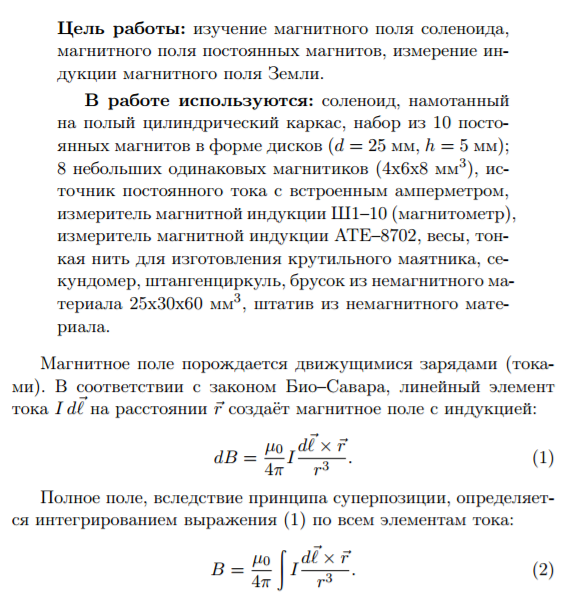
\includegraphics[width=15cm]{theory1.png}
       	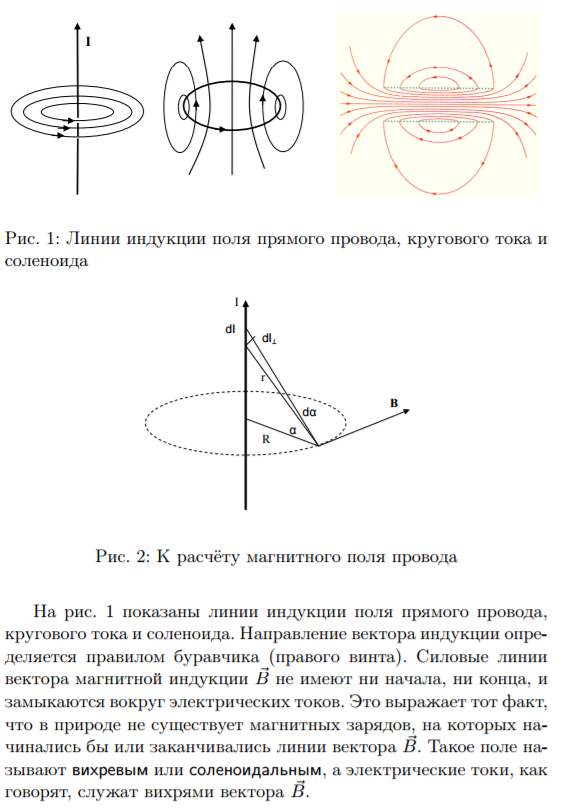
\includegraphics[width=15cm]{theory2.png}
       	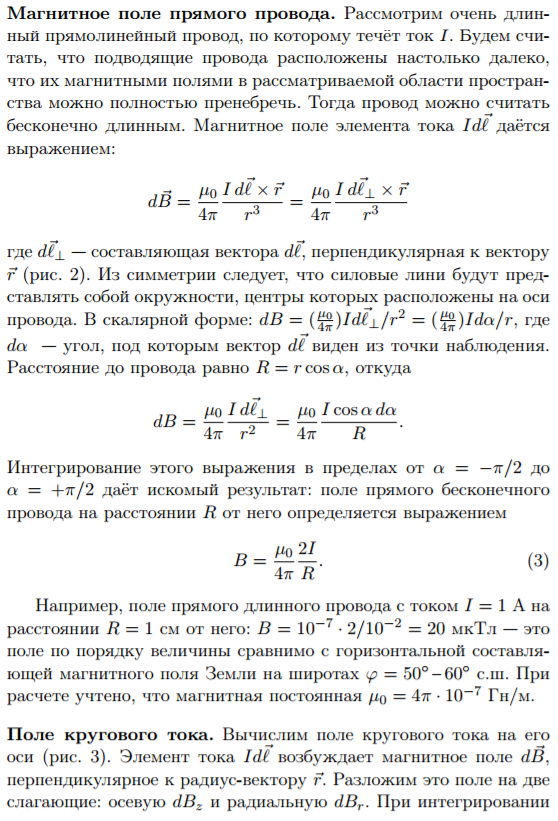
\includegraphics[width=15cm]{theory3.png}
       	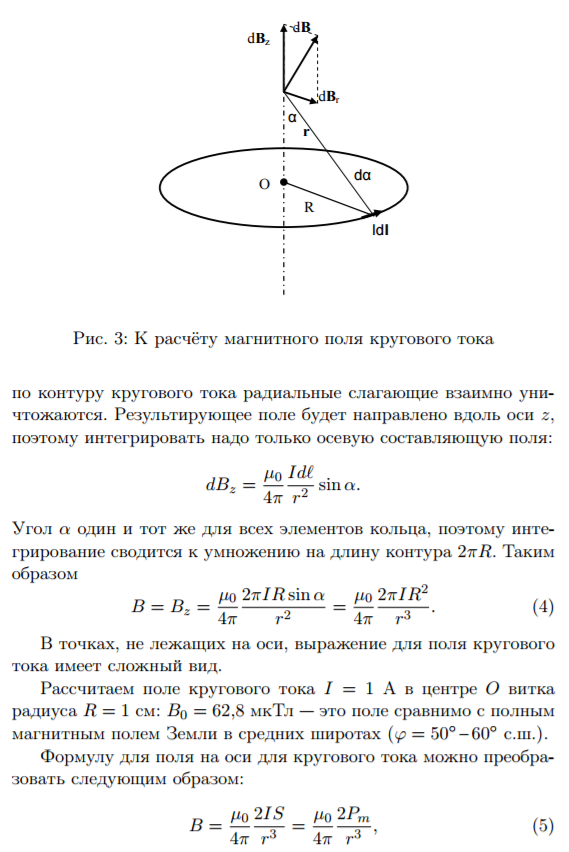
\includegraphics[width=15cm]{theory4.png}
       	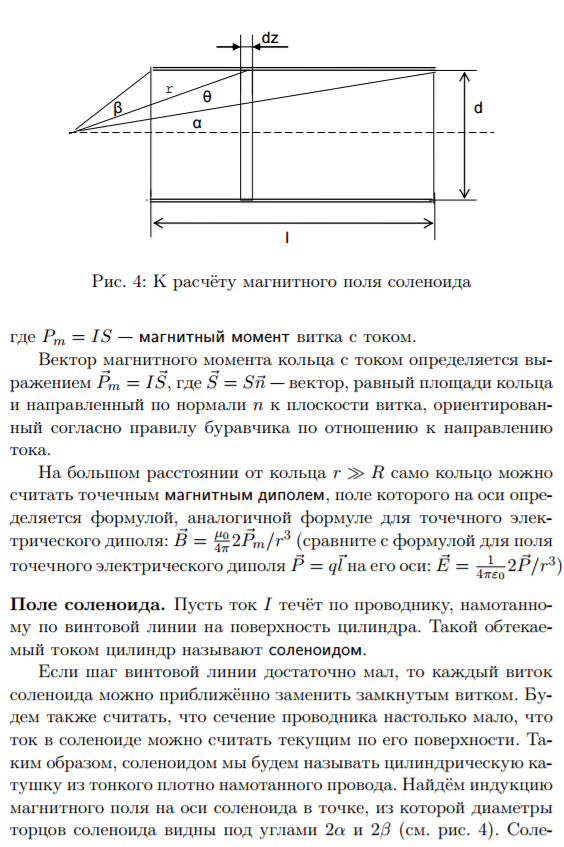
\includegraphics[width=15cm]{theory5.png}
        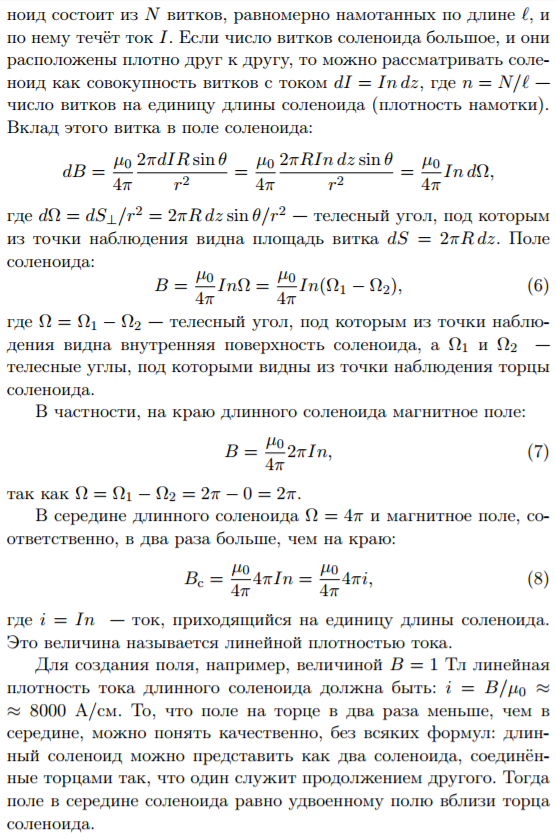
\includegraphics[width=15cm]{theory6.png}
	    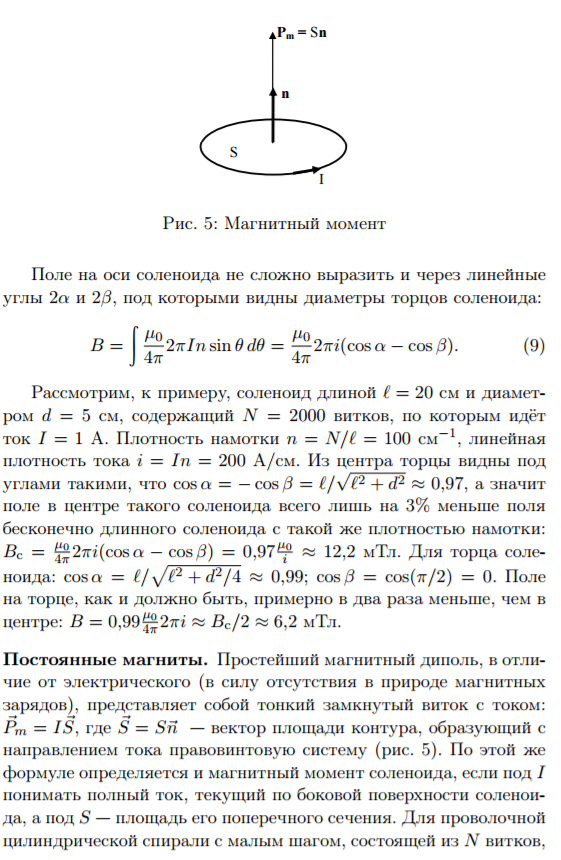
\includegraphics[width=15cm]{theory7.png}
	    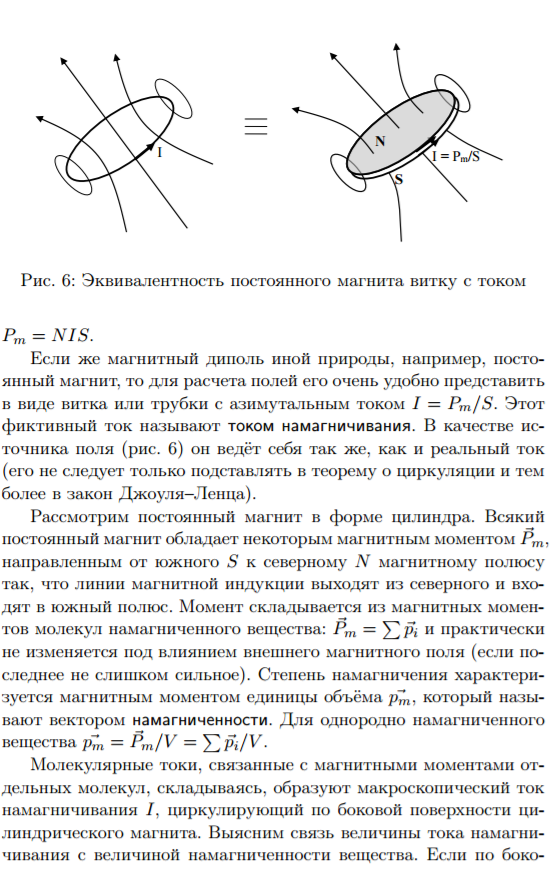
\includegraphics[width=15cm]{theory8.png}
	    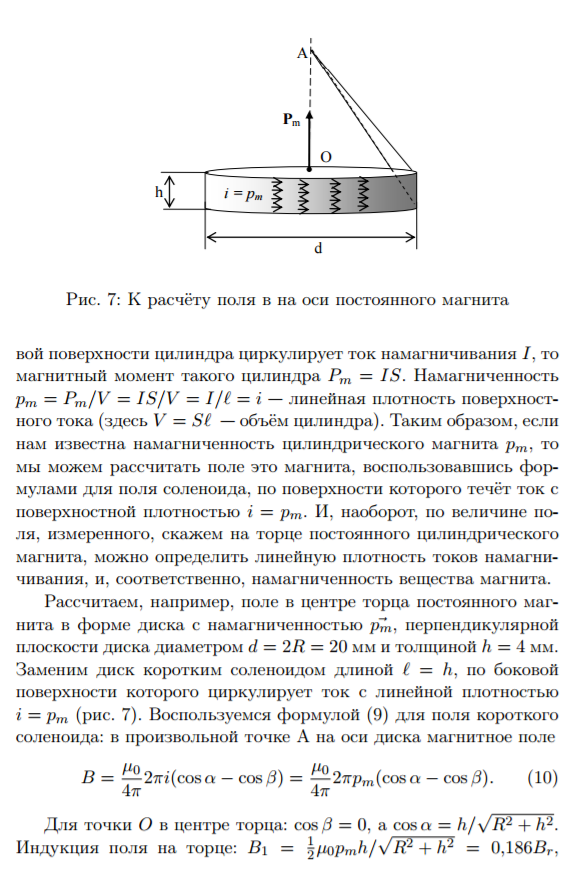
\includegraphics[width=15cm]{theory9.png}
	    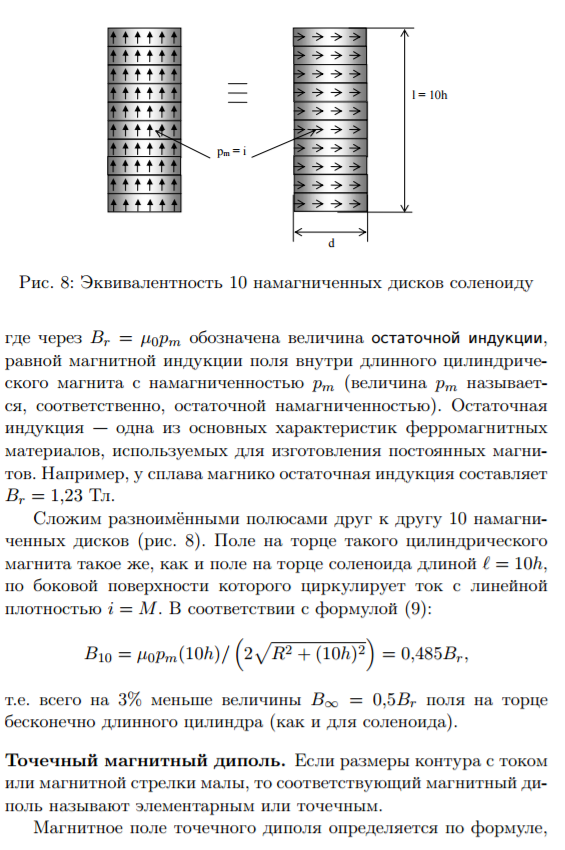
\includegraphics[width=15cm]{theory10.png}
	    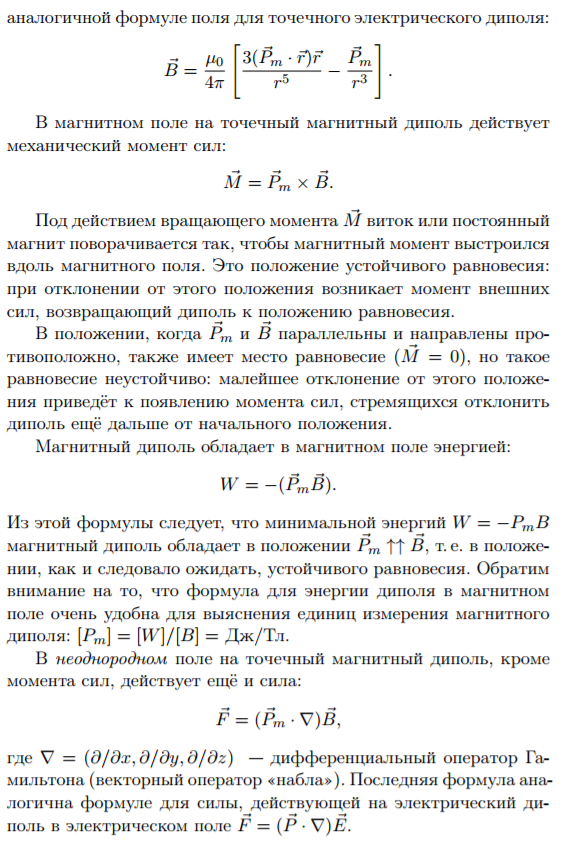
\includegraphics[width=15cm]{theory11.png}
	    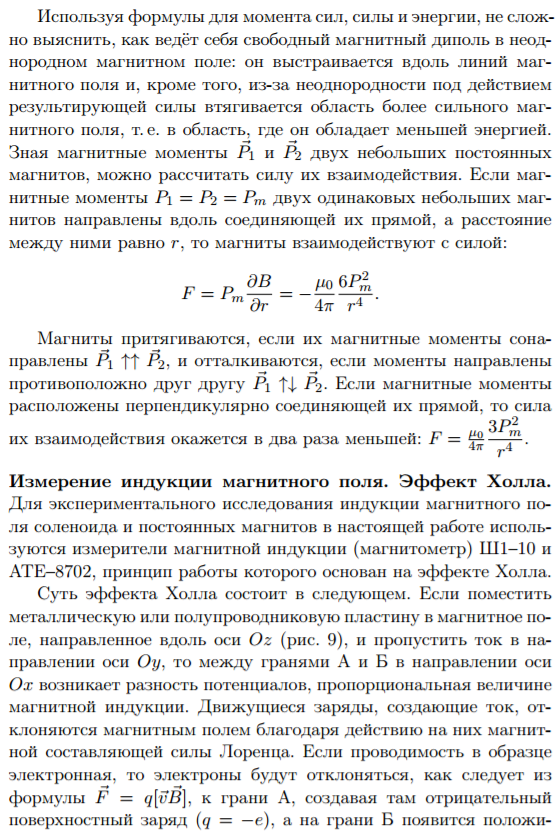
\includegraphics[width=15cm]{theory12.png}
	    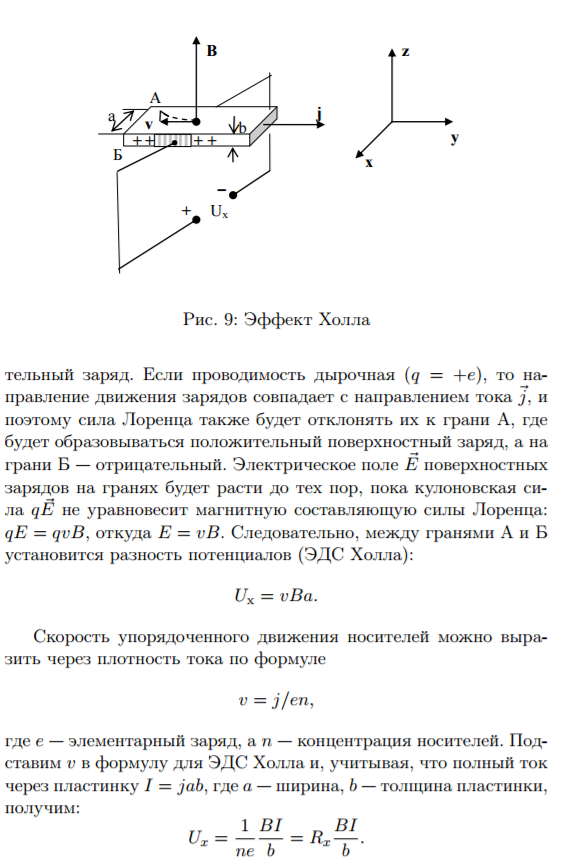
\includegraphics[width=15cm]{theory13.png}
	    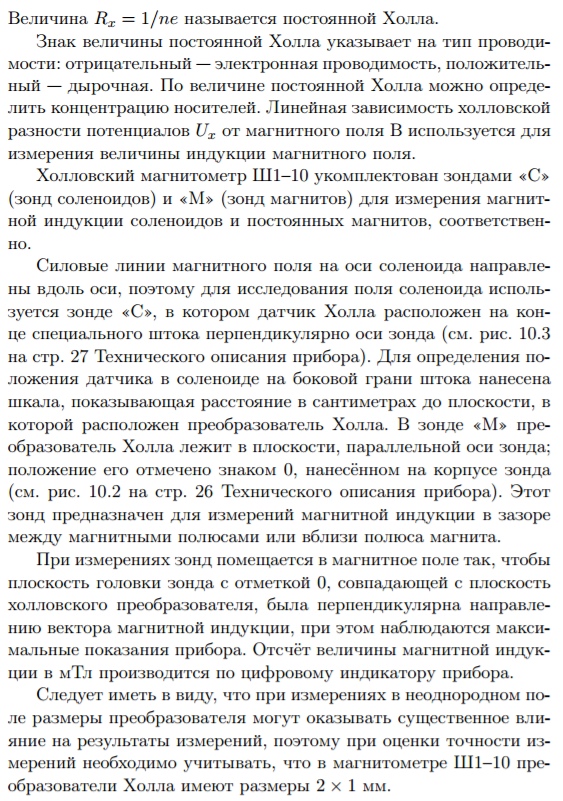
\includegraphics[width=15cm]{theory14.png}
	    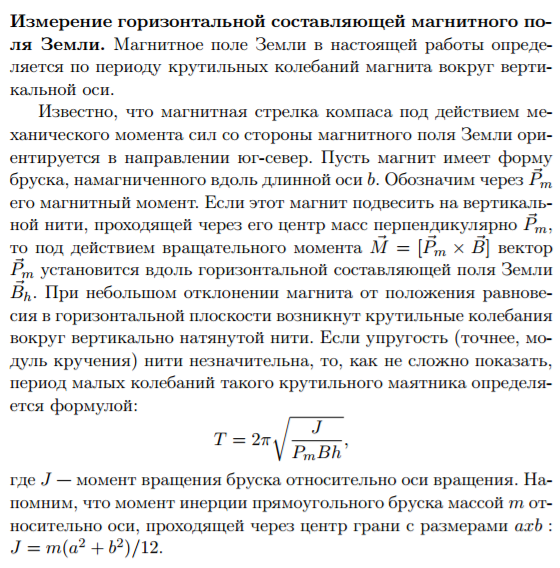
\includegraphics[width=15cm]{theory15.png}
    \end{center}
    
    \begin{center}
    	\textbf{\large Выполнение работы.}
    \end{center}
    
    \textbf{\large Часть А}
    \newline
    
    Подключаем к магнитометру зонд, включаем магнитометр. Ждём установления рабочего режима. После установления рабочего режима включаем источник питания соленоида и устанавливаем ток в соленоиде $I = 0,5 A$.
    
    Будем перемещать зонд вдоль оси соленоида с интервалом 0,5 см, снимая зависимость индукции магнитного поля от координаты z. Считаем $\sigma_z = 2 мм$, $\sigma_B = 0,01 мТл$. Результаты в таблице:
    
    \begin{center}
    	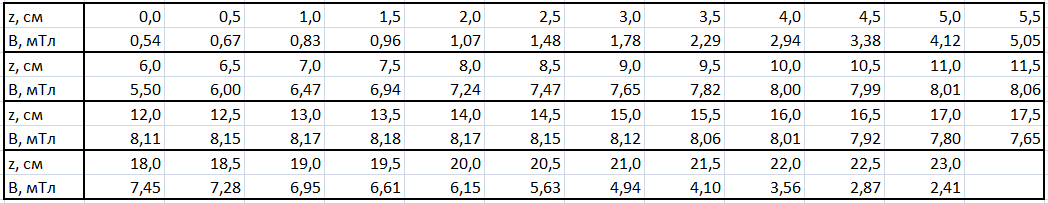
\includegraphics[width=16cm]{table1.png}
    \end{center}
    
    Построим график:
    
    \begin{center}
    	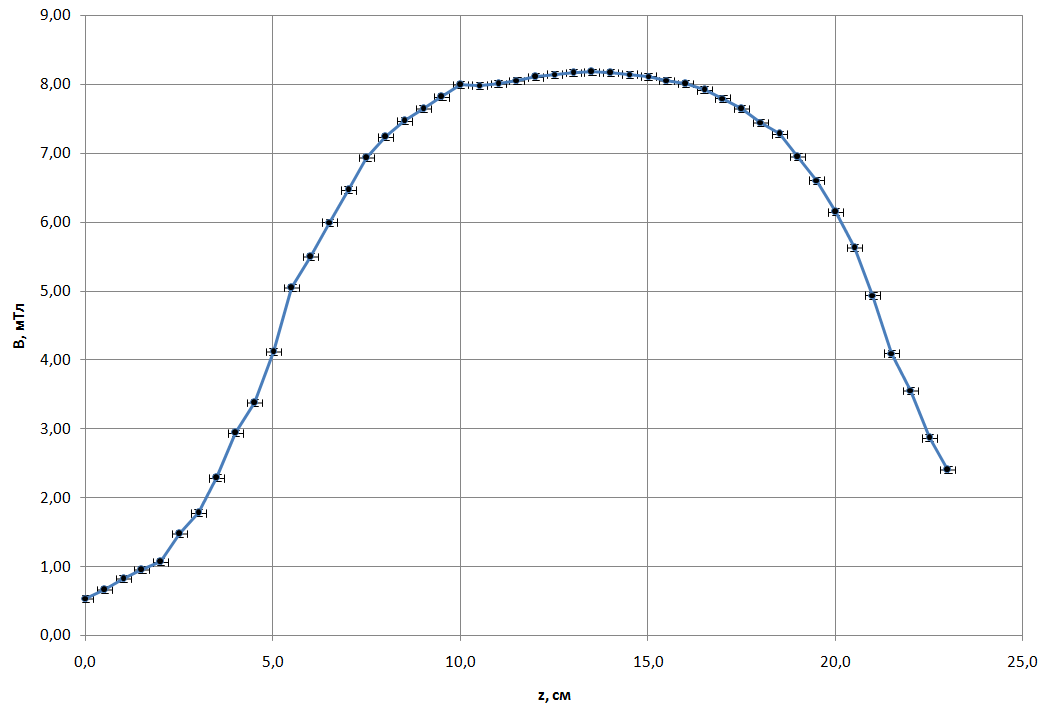
\includegraphics[width=18cm]{graph1.png}
    \end{center}
    
    По максимальному значению индукции определим координату средней точки на оси соленоида. $z=13,5 \pm 0,3 cм$.
    
    Поместив зонд в среднюю точку, снимем зависимость $B(I)$, изменяя $I$ от 0,5А до 2,5А. При измерениях $\sigma_I = 0,05A$, $\sigma_B = 0,1мТл$.
    
    \begin{center}
    	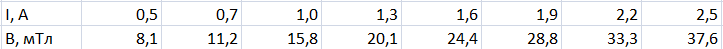
\includegraphics[width=18cm]{table2.png}
    	\newpage
    	Построим график:
    	
    	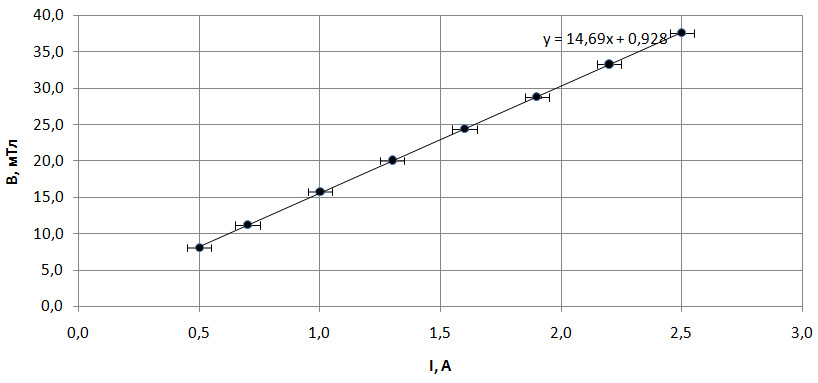
\includegraphics[width=18cm]{graph2.png}
    \end{center}
    
    Найденный коэффициент наклона $k = 14,7 \pm 0,2 мТл/А$, из теории же $B = \frac{4\pi}{c}\frac{N}{l} I$
    
    Оценим теперь длину и количество витков соленоида. Поле на границе соленоида должно быть в 2 раза меньше поля в центре, таким образом $l = 2(z_{ср} - z_{кр}) = 17,0 \pm 0,7 см$. 
    
    Теперь найдём плотность намотки $n$, используя график $B(I)$ - $B(I) = \mu_0nI$. Итак, $n = \frac{k}{\mu_0} = (11,7 \pm 0,2) * 10^3 м^{-1}$
    
    Отсюда $N = nl = (1,9 \pm 0,2) * 10^3$.
    
    Реальные значения $N = 2300$, $l = 16,7 см$. С точностью $2\sigma$ совпадают с вычисленными.
    
    Теоретическая зависимость (рассчитана только внутри соленоида) $B(z) = \frac{NI}{cl}*2\pi (1 + \frac{h(z)}{R^2 + h(z)^2})$, где $h(z) = \frac{l}{2} - |\frac{l}{2} - z|$. Здесь h - расстояние до ближайшего конца соленоида, R = 3,5/2 см - радиус кольца соленоида, N - количество витков, l - длина соленоида.\\
    
    \textbf{\large Часть Б}
    \newline
    
    Измерим индукцию магнитного поля в центре постоянного магнита в форме диска.
    Теперь будем складывать цилиндр из n дисков и измерим зависимость магнитной
    индукции в центре торца цилиндра от числа магнитов, образующих цилиндр. При измерениях $\sigma_B = 1мТл$.
    
    \begin{center}
    	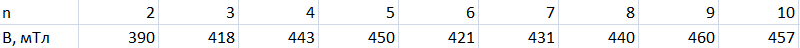
\includegraphics[width=15cm]{table3.png}
    	
    	\pagebreak
    	Построим график:
    	
    	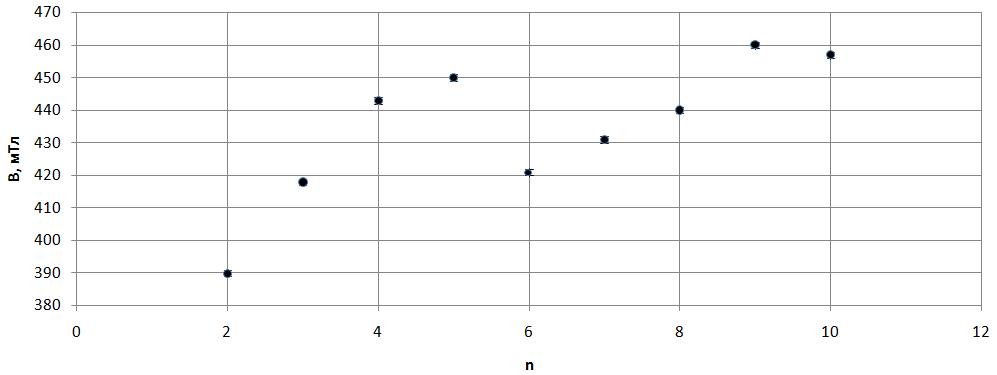
\includegraphics[width=15cm]{graph3.png}
    \end{center}
    
    Найденный коэффициент наклона $k = (6,2 \pm 0,7) * 10^-3 мТл$
    
    Теоретическая зависимость: $B(n) = \mu_0 p_m \frac{nh}{2\sqrt{R^2 + (nh)^2}}$, h = 0,5см - толщина одного магнита, R = 0,5см - радиус.
    
    \begin{center}
    	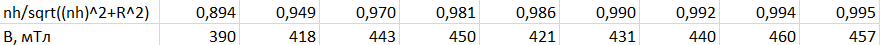
\includegraphics[width=15cm]{table4.png}
    	
    	Построим график:
    	
    	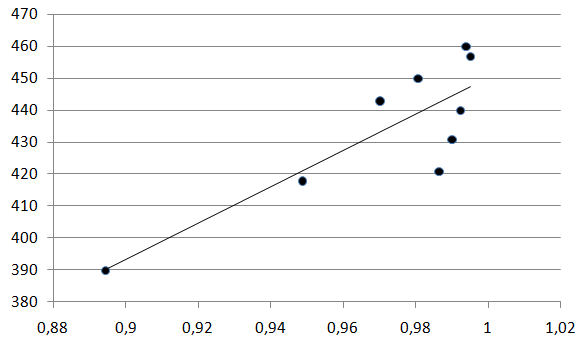
\includegraphics[width=15cm]{graph4.png}
    \end{center}
    
    Найденный коэффициент наклона $k = (59 \pm 3)*10 мТл$
    Отсюда находим остаточную намагниченность $B = 295 \pm 15 мТл$.\\
    
    \textbf{\large Часть В}
    
    Положим между двумя магнитами брусок из бумаги — немагнитного материала.
    Получим максимальное расстояние, на котором магниты удерживают друг друга
    в поле тяжести земли: $r_max = 1,83 см$.
    
    Взвесим оба магнита: $m_1 = 0,868 g$, $m_2 = 0,866 g$.
    
    Теперь вычислим магнитный момент $\frac{\mu_0}{4\pi}\frac{6P_m^2}{r_{max}^4} = mg$
    
    $P_m = (3,98 \pm 0,01) * 10^{-2} А*м$
    
    Намагниченность $p_m = \frac{P_m}{V} = (1,01 \pm 0,02) * 10^5 А/м$.
    
    Остаточная магнитная индукция: $B_r = \mu_0 p_m = 12,6 \pm 0,03 мТл$\\
    
    \textbf{\large Часть Г}\\
    
    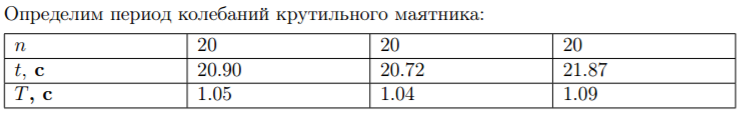
\includegraphics[width=15cm]{res1.png}\\
    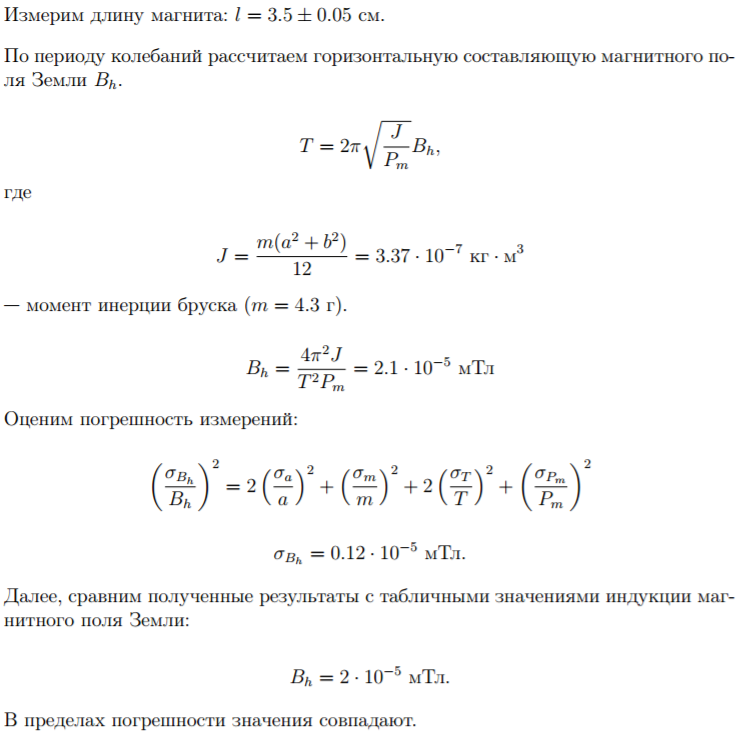
\includegraphics[width=15cm]{res2.png}
\end{document}